\section{Background}
People have been playing mathematical games
since as early as 2000 B.C.
\cite{cornelius1986historical}.
From the beginning,
players have attempted to devise optimal
strategies, simulate future moves, or identify
flaws that can be exploited.
Mathematics can serve as a particularly powerful tool for
such analysis.
Abbott and Richey used Markov Chains
to find the long term 
distribution of turns players spend in different
properties in the board game
\textit{Monopoly} \cite{abbott1997take, magie1935}.
(They also found that the optimal strategy is to avoid making
moves altogether and instead maximize time spent in jail.)
Lyford et al. investigated the probability and expected value 
in the board game \textit{Camel Up}
\cite{bogen2014, lyford2019using}.
Witter and Lyford generated an optimal winning strategy for the 
board game \textit{Codenames} using matrix rotations
and a combinatorial argument \cite{chvatil2015}.
% TO DO: CITE CODENAMES PAPER IF ACCEPTED

Another example of a game with mathematical underpinnings is
the board game \textit{Ticket to Ride} \cite{moon2004ticket}. 
Players race to connect 
cities and build railroads on a map of the U.S.
Mathematically, the board
can be thought of as a graph where
cities represent vertices and the
routes between them represent edges.
The educational implications of \textit{Ticket to Ride}
have been extensively studied.
Lim applied the game to teach basic graph theory
\cite{lim2007taking}.
Chang et al. introduced Kruskal's, Prim's, and Dijkstra's
algorithms in the context of \textit{Ticket to Ride}
\cite{chang2008learning}.
Drake taught beginning programming skills by having
students implement a digital version of the game \cite{drake2011teaching}.
In addition, \textit{Ticket to Ride} has been studied in the context of
accessible game design and eye-tracking visualization
\cite{eriksson2005enhancing, newn2017evaluating}.

Previous work has also focused on improving player 
strategies in \textit{Ticket to Ride}.
Silva et al. used simulations to compare different
heuristic strategies (e.g. purchasing longest routes,
connecting all destination cards) \cite{de2017playtesting}.
In related papers, the same authors explore the 
game space to find trends in the way \textit{Ticket to Ride}
is played and experiment with new maps and decks 
\cite{de2017evaluator, de2018evolving}.

We extend the mathematical interpretations of
\textit{Ticket to Ride} to build on previous research
and devise better player strategies.
In particular, we apply expected value of collecting cards,
effective resistance, and betweenness centrality.

We rely on a well-known solution to the probability question:
"What is the expected number of cards until
we see three aces in a well-shuffled deck?"
We frame the problem of collecting the resources
to build a route in terms of the aces problem.
The solution gives us a proxy for the difficulty
of collecting routes.

In a graph, effective resistance corresponds
to the difficulty of an electrical current flowing
from one vertex to another.
We implement two existing algorithms to calculate
the effective resistances between cities
\cite{ellens2011effective, wu2004theory}.
By comparing the effective resistance to the reward
of collecting a pair of cities, we suggest an enhanced approach 
approach to picking destination cards.

Developed in 1977, betweenness centrality gives a measure
of the centrality of edges in a graph
\cite{freeman1977set}.
By calculating the edges with the highest betweenness centrality,
we enable players to pick the most central routes.
We compare the most theoretically central routes
to the ones owned by the winning player in Silva et al.'s
simulations \cite{de2017playtesting}.

The overarching question of this work is as follows:
What (if any) mathematical structure in \textit{Ticket to Ride}
can be exploited to optimize player strategies?
Our answer builds on existing results and
and our own novel applications of mathematical concepts to enhance
player strategies and propose a better scoring scheme.

\begin{figure}[h]
\centering
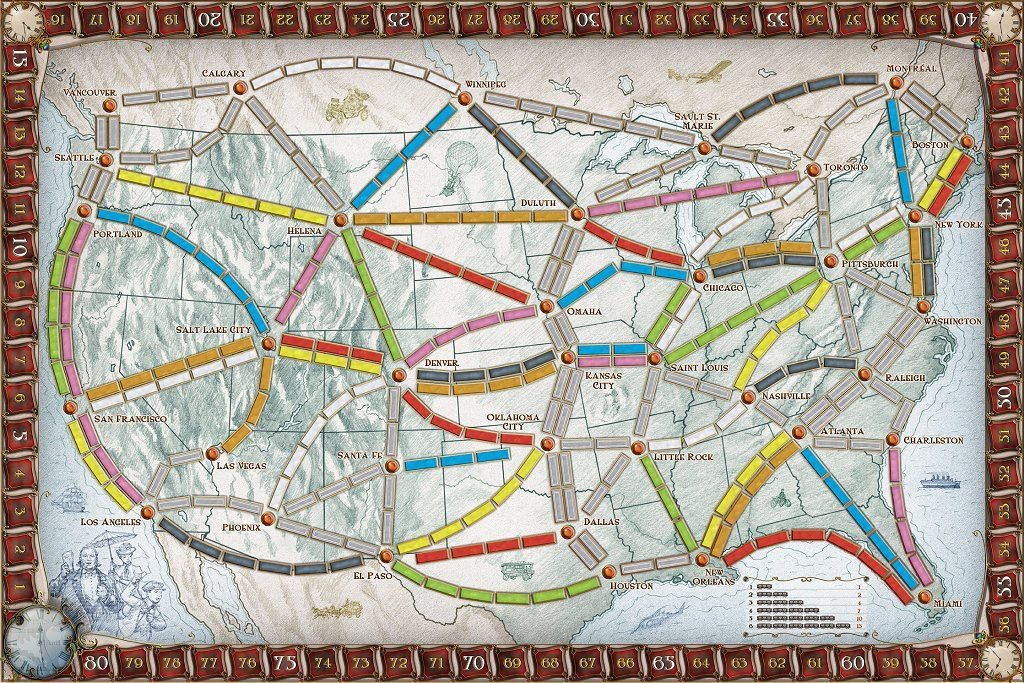
\includegraphics[scale=.25]{figures/board}
\caption{The \textit{Ticket to Ride} U.S. board.}
\end{figure}

\subsection{Ticket to Ride}
The goal is to collect as many points as possible before
any player uses all of their 45 trains and ends the game.
There are three ways players may earn points:
1) by building routes on the board
according to the number of trains in each route,
2) by building a path of routes
between two cities specified by a destination card in their possession,
3) by owning the longest continuous path of cities at the end of the game.

A player has three (mutually exclusive) options for what to do during
their turn:
1) draw train cards to build routes in later turns,
2) claim a particular route by returning the appropriate
number of trains of the specified color,
3) draw destination cards in order to earn points for connecting
distant cities.
\subsection{Strategy Assumptions}
We make several assumptions about how reasonable players
play \textit{Ticket to Ride}.